\section{Certyfikaty SSL/TLS}

\begin{frame}{SSL/TLS}
	\begin{figure}
		\centering
		

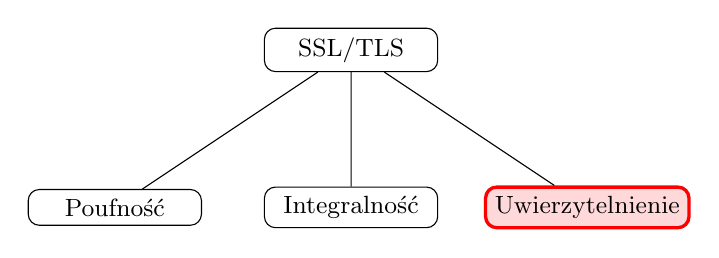
\begin{tikzpicture}[
		level distance=20mm,
		sibling distance=30mm,
		every node/.style={
				draw,
				rounded corners,
				align=center,
				minimum width=22mm,
				font=\small
			},
		highlight/.style={
				draw=red,
				very thick,
				fill=red!15
			}
	]
	\node {SSL/TLS}
	child { node {Poufność} }
	child { node {Integralność} }
	child { node[highlight] {Uwierzytelnienie} };
\end{tikzpicture}

		\caption{SSL/TLS gwarantuje poufność, integralność i uwierzytelnienie.}
	\end{figure}
\end{frame}

\begin{frame}{SSL/TLS - uwierzytelnienie}
	\begin{itemize}
		\item SSL/TLS używa certyfikatów X.509
		\item Certyfikaty są wydawane przez zaufane podmioty zwane Urzędami Certyfikacji (CA).
		\item Przeglądarka posiada listę zaufanych CA
		\item Certyfikat jest zweryfikowany jeśli:
		      \begin{itemize}
			      \item jest ważny
			      \item został wydany przez zaufanego CA
		      \end{itemize}
	\end{itemize}
\end{frame}

\begin{frame}{SSL/TLS - certyfikaty X.509}
	\begin{itemize}
		\item Certyfikat X.509 zawiera (między innymi):
		      \begin{itemize}
			      \item Nazwę podmiotu (np. nazwę domeny).
			      \item Klucz publiczny podmiotu.
			      \item Dane o wydającym CA.
			      \item Data wystawienia certyfikatu.
			      \item Okres ważności certyfikatu.
			      \item Podpis cyfrowy wydającego CA.
		      \end{itemize}
	\end{itemize}
\end{frame}

\begin{frame}{SSL/TLS - weryfikacja certyfikatu}
	\begin{itemize}
		\item Przeglądarka musi zweryfikować certyfikat domeny, sprawdzając:
		      \begin{itemize}
			      \item Czy certyfikat jest podpisany przez zaufanego CA.
			      \item Czy nazwa domeny w certyfikacie pasuje do odwiedzanej strony.
			      \item Czy certyfikat nie wygasł.
			      \item Czy certyfikat nie został unieważniony (CRL, OCSP).
		      \end{itemize}
		\item Trzeba również sprawdzić certyfikaty pośrednie w łańcuchu zaufania.
	\end{itemize}
\end{frame}

\begin{frame}{SSL/TLS - Podatności}
	\begin{itemize}
		\item Podatności weryfikacji w SSL/TLS mogą wynikać z:
		      \begin{itemize}
			      \item Błędów implementacji weryfikacji SSL/TLS.
			      \item Słabych algorytmów kryptograficznych (np. RC4, MD5).
		      \end{itemize}
		\item Przy błędniej weryfikacji, atak MitM staje się możliwy, nawet przy użyciu SSL/TLS.
	\end{itemize}
\end{frame}
